\documentclass{ximera}
\title{Implicit Differentiation - Finish solutions}
\begin{abstract}
\end{abstract}
\begin{document}
\maketitle
\begin{image}
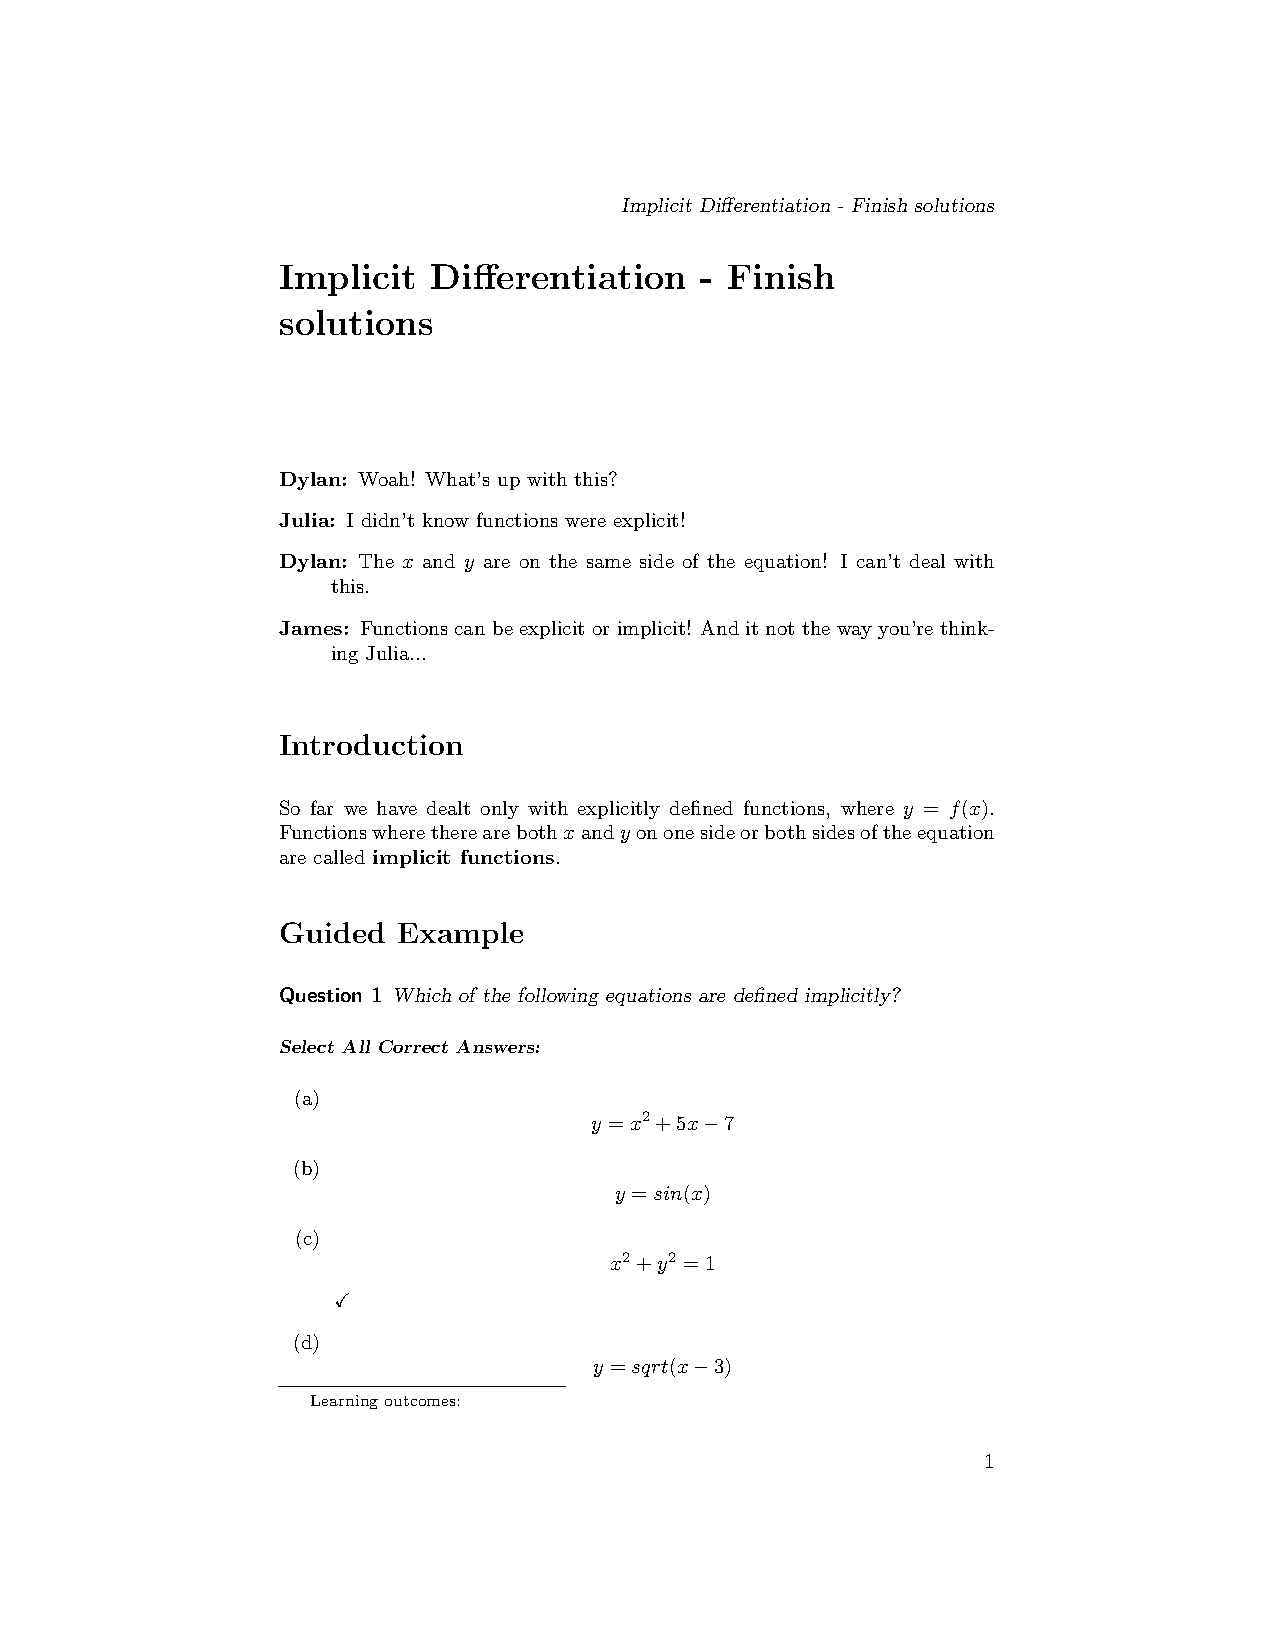
\includegraphics{implicit_differentiation}
\end{image}
\begin{dialogue}
\item[Dylan] Woah! What's up with this?
\item[Julia] I didn't know functions were explicit!
\item[Dylan] The $x$ and $y$ are on the same side of the equation! I can't deal with this.
\item[James] Functions can be explicit or implicit! And it not the way you're thinking Julia...
\end{dialogue}
\section{Introduction}
So far we have dealt only with explicitly defined functions, where $y=f(x)$.  Functions where there are both $x$ and $y$ on one side or both sides of the equation are called \textbf{implicit functions}.
\section{Guided Example}
\begin{question}
Which of the following equations are defined implicitly?
\begin{selectAll}
\choice{$$y=x^2+5x-7$$}
\choice{$$y=\sin(x)$$}
\choice[correct]{$$x^2+y^2=1$$}
\choice{$$y=\sqrt(x-3)$$}
\choice[correct]{$x^2y^3+y = 5x+8y$}
\end{selectAll}
\end{question}
Graph the following implicitly defined function below, $$x^2+y^2=1$$
\[
\graph{}
\]
Now, in the following sage cell, solve the function for y. For help using the solve command refer to the \href{http://doc.sagemath.org/html/en/tutorial/tour_algebra.html#solving-equations}{documentation} here.
\begin{onlineOnly}
\begin{sageCell}
x,y = var("x, y")
#eqn = x**2+y**2==1, this sets eqn to the unit circle
#use the solve command to solve eqn for y
\end{sageCell}
\end{onlineOnly}
Graph the two explicit equations on the same axis below.
\[
\graph{}
\]
\begin{question}
Which of the following are true?
\begin{selectAll}
\choice{$x^2+y^2=1$ is a function}
\choice[correct]{$y=-\sqrt{1-x^2}$ is a function}
\choice[correct]{$y=\sqrt{1-x^2}$ is a function}
\end{selectAll}
\end{question}

\begin{question}
\begin{onlineOnly}
\begin{sageCell}

\end{sageCell}
\end{onlineOnly}
Using the functions you found, differentiate to find the slope of the tangent lines at the point $\left(\frac{\sqrt{2}}{2}\right),\left(\frac{\sqrt{2}}{2}\right)$. You may do this in the above sage cell or by hand.
$\answer{-1}$
\end{question}
Unfortunately not all implicit equations can be easily solved for y, which is why we use implicit differentiation! If you are familiar with implicit differentiation you can skip the following explanation.
\begin{explanation}
Starting with
$$x^2 + y^2 = 1$$
we first differentiate each term using $\frac{d}{dx}$
$$\frac{d}{dx}x^2+\frac{d}{dx}y^2 = \frac{d}{dx} 1$$
You can already fill in 2 of the terms
$$ \answer{2x}+ \frac{d}{dx}y^2 = \answer{0}$$
For the term $\frac{d}{dx} y^2$ you can imagine $y = f(x)$, and hence by the chain rule
 $$\frac{d}{dx} y^2 = \frac{d}{dx}(f(x))^2 $$ \\
 $$= 2\cdot f(x) \cdot f'(x) $$ \\
 $$= 2y\frac{dy}{dx}$$ \\
 Putting this together we have
 $$2x + 2y\frac{dy}{dx} =0$$
Solving for $\frac{dy}{dx}$ we get 
$$\answer{\frac{-x}{y}}$$
\end{explanation}
\begin{question}
Use the equation obtained from the above explanation to find $\frac{dy}{dx}$ at $\left(\frac{\sqrt{2}}{2}\right),\left(\frac{\sqrt{2}}{2}\right)$ 
$\answer{-1}$
\begin{feedback}
Using both methods you can obtain the same answer, but for some equations the first method is much more work!
\end{feedback}
\end{question}
\section{On Your Own}
Consider the equation $y^4+xy=x^3-x+2$.
\begin{onlineOnly}
\begin{sageCell}
x,y=var('x','y')
f(x,y) = x^3 + y^3 - 6*x*y

y=function('y',x)
temp=diff(f(x,y))
solve(temp,diff(y))

\end{sageCell}
\end{onlineOnly}

\begin{question}
Using your result in the previous section, evaluate $\frac{dy}{dx}$ at $x = 3$ and $x = 7$.

$x = 3: \answer{}$

$x = 7: \answer{}$
\end{question}
\begin{question}
\begin{onlineOnly}
\begin{sageCell}
var("x, y")

\end{sageCell}
\end{onlineOnly}

Now use Sage Math to find the slope of  $\sin(x^2)=\cos(xy^2)$ at any point. \href{http://doc.sagemath.org/html/en/tutorial/tour_algebra.html#differentiation-integration-etc}{Look here for information on implicit differentiation in Sage}
$\answer{}$
\end{question}
\section{Perpendicular at a Point}
\begin{dialogue}
\item[Julia] Wow, implicit differentiation is rough.
\item[Dylan] You're telling me... I've been doing this for hours! I wish we could at least do a little more with it if I have to learn it.
\item[James] Did I hear that you guys want to know more about using implicit differentiation?
\item[Julia and Dylan] James! Tell us more!
\item[James] Alright guys, you can use implicit differentiation with implicit functions to tell if two functions are perpendicular at a point!
\item[Julia] But how?
\item[Dylan] Yeah, I don't see how that helps.
\item[James] It's easy - all we have to do is see if the tangent lines are perpendicular at that point, and if they are, then so are the curves!
\end{dialogue}
\begin{question}
Graph $3x - 2y + x^3-x^2y = 0$ and $x^2 - 2x + y^2 - 3y = 0$ on the same set of axes.
\[
\graph{}
\]

Do they look perpendicular anywhere?
$\answer{Yes}$
\end{question}
\begin{question}
\begin{hint}
To show two lines are perpendicular you must show that the slope of one is the opposite inverse of the other
\end{hint}
Show the two curves are (or are not) perpendicular at the origin. You can do this in the sage cell provided or by hand.
\begin{onlineOnly}
\begin{sageCell}

\end{sageCell}
\end{onlineOnly}
Slope of $3x - 2y + x^3-x^2y = 0$ at the origin $\answer{3/2}$
Slope of $x^2 - 2x + y^2 - 3y = 0$ at the origin $\answer{-2/3}$
Are the lines perpendicular at the origin?



\end{question}
\section{In Summary}
There are two main methods to solve implicit equations
\begin{enumerate}
\item{Solve for $y$ and then differentiate.}
\item{Treat $y$ as $y(x)$ and differentiate for $x$, eventually solving for $\frac{dy}{dx}$ to give the value of the derivative at any point.}
\end{enumerate}
\pagebreak
\end{document}
